\documentclass[preprint,12pt]{elsarticle}

\usepackage{amsmath,amssymb,amsfonts}
\usepackage{graphicx}
\usepackage{booktabs}
\usepackage{tabularx}
\usepackage{multirow}
\usepackage{array}
\usepackage{makecell}
\usepackage{float}
\usepackage[section]{placeins}
\usepackage{dirtree}
\usepackage{tcolorbox}
\usepackage{hyperref}
\usepackage{url}
\usepackage{xcolor}
\usepackage{geometry}
\usepackage{tikz}
\geometry{a4paper, margin=1in}

% Cấu hình hiển thị cây thư mục dirtree thanh lịch
\renewcommand*\DTstylecomment{\rmfamily\color{blue!70!black}\footnotesize\itshape}
\renewcommand*\DTstyle{\ttfamily\small}

% Tối ưu hóa phân bố float của LaTeX (ngăn chặn trôi dạt bảng/hình)
\renewcommand{\topfraction}{0.95}
\renewcommand{\bottomfraction}{0.85}
\renewcommand{\textfraction}{0.05}
\renewcommand{\floatpagefraction}{0.75}
\setcounter{topnumber}{4}
\setcounter{bottomnumber}{3}
\setcounter{totalnumber}{6}

\journal{Data in Brief}

% ORCID icon macro
\newcommand{\orcidicon}[1]{\href{https://orcid.org/#1}{\texorpdfstring{%

\begin{tikzpicture}[baseline=-0.4ex]%
\draw[fill=lime!80!black,draw=none] (0,0) circle (0.9ex);%
\node at (0,0) {\color{white}\fontsize{3.5}{3.5}\selectfont\sffamily\bfseries iD};%
\end{tikzpicture}%
}{}}}

\begin{document}

\begin{frontmatter}

\title{HCMC-TrafficSnap: A City-Scale Multi-Camera Image Time-Series and Directed Spatial Graph Dataset for Heterogeneous Urban Traffic}

\author[inst1]{Viet-Anh Le \orcidicon{0009-0003-5748-0439}}
\ead{anhlv.b23kh002@stu.ptit.edu.vn}

\author[inst1]{Khanh Nguyen-Trong \orcidicon{0000-0001-5175-8805}\corref{cor1}}
\ead{khanhnt@ptit.edu.vn}

\cortext[cor1]{Corresponding author.}
\affiliation[inst1]{organization={Intelligent Computing for Sustainable Development Laboratory (IC4SD), Posts and Telecommunications Institute of Technology (PTIT)},
            city={Hanoi},
            country={Vietnam}}

\begin{abstract}
This data article presents \textbf{HCMC-TrafficSnap}, an open-access multimodal dataset comprising 714,123 discrete surveillance camera snapshots (44.38~GB total storage volume) coupled with an OpenStreetMap-derived directed road routing distance graph across 608 indexed traffic surveillance stations in Ho Chi Minh City, Vietnam (572 continuous active stations yielding 1,250--1,268 frames each, and 36 stations with initial upstream stream dropouts). Collected continuously over 93.6 hours (3.9 calendar days, from 02/10/2026 17:37 to 06/10/2026 15:12 ICT) at an empirical mean sampling interval of $\Delta T = 269.0 \pm 239.7$~s (median: $263.0$~s; nominal target: 5.0 minutes), the dataset addresses a notable empirical gap in Intelligent Transportation Systems: the absence of large-scale observational visual time-series capturing heterogeneous, motorcycle-dominant metropolitan traffic flows (where two-wheeled vehicles comprise 70--80\% of modal volume). All visual records are provided in standard $512 \times 288$ pixel JPEG format (average file size $65.17 \pm 13.36$~KB), with an empirical acquisition clock offset of $\Delta t_{\text{lag}} = 15.0 \pm 4.2$~s relative to hardware camera clocks. The visual time-series is paired with a $608 \times 608$ directed topological routing matrix containing 2,450 valid corridors within a 6.0~km spatial cutoff horizon, exhibiting marked directional asymmetry (1,070 strictly one-way pairs and 238 distance-asymmetric bidirectional pairs) due to median barriers and one-way arterial regulations. Production-grade PyTorch data loaders, multi-camera self-supervised batch samplers, and dual-transition directed graph utilities are provided. Quantitative privacy audits across 2,000 sampled images confirm that due to camera elevation ($>6$~m) and sub-Nyquist ground sampling distance ($2.73 - 3.25$~cm/px), no individual faces or license plates are resolvable (0.00\% leakage).
\end{abstract}

\begin{keyword}
Intelligent Transportation Systems \sep Image Time-Series \sep Traffic Camera Snapshots \sep Unlabeled Surveillance Data \sep Spatio-Temporal Graph Networks \sep Mixed Urban Traffic
\end{keyword}

\end{frontmatter}

%% Specifications Table (Table 1 - Trình bày trang trọng trên trang riêng theo chuẩn Elsevier Data in Brief)
\clearpage
% Table 1: Specifications Table (Elsevier Data in Brief Standard Template)
\begin{table*}[!htbp]
\centering
\small
\setlength{\tabcolsep}{6pt}
\renewcommand{\arraystretch}{1.15}
\caption{Specifications Table of the IC4SD-TrafficSnap Dataset.}
\label{tab:specifications}
\begin{tabularx}{\textwidth}{@{} >{\raggedright\arraybackslash\bfseries}p{4.2cm} >{\raggedright\arraybackslash}X @{}}
\toprule
Subject & Computer Science \\
\midrule
Specific subject area & Intelligent Transportation Systems, Computer Vision, Spatio-Temporal Data Mining \\
\midrule
Type of data & Image time-series, geospatial metadata, derived road network graph tensors, PyTorch code utilities \\
\midrule
How data were acquired & Automated retrieval from the public municipal traffic surveillance portal of the Ho Chi Minh City Department of Transportation (\url{https://giaothong.hochiminhcity.gov.vn}) via asynchronous HTTP polling. Driving distances and road network routing were computed using OSRM over OpenStreetMap data. \\
\midrule
Data format & Raw snapshots: RGB JPEG ($512 \times 288$ px, JFIF 1.01, stream quality factor $\approx 75$--$80$); \newline
Geospatial metadata: Tabular CSV (\path{routes.csv}, \path{stations.csv}, \path{road_network_distance.csv}); \newline
Graph tensors: NumPy binary arrays (\path{distance_km.npy}, \path{direction.npy}) and tabular edge list (\path{edges.csv}); \newline
Code: Python source files (\path{code/}). \\
\midrule
Description of data collection & Snapshots were collected across $608$ indexed surveillance stations in Ho Chi Minh City over $93.6$ continuous hours (October 2, 2026, 17:37 to October 6, 2026, 15:12 ICT) with an empirical sampling interval of $\Delta T = 269.0 \pm 239.7$~s (median: $263.0$~s). Camera positions are mapped to OpenStreetMap road geometry, yielding a derived directed spatial graph with $2,450$ corridor links within a $6.0$~km driving cutoff horizon. \\
\midrule
Data source location & Region: Ho Chi Minh City, Vietnam (former urban districts, core metropolitan area); \newline
Coordinates: $[10.68^\circ\text{N} - 10.88^\circ\text{N}, 106.58^\circ\text{E} - 106.82^\circ\text{E}]$. \\
\midrule
Data accessibility & Repository name: Zenodo; \newline
Direct URL: \url{https://doi.org/10.5281/zenodo.22929940} (Release v2.0); \newline
Licensing: Surveillance imagery and metadata are released for non-commercial academic research; derived road graph is licensed under the Open Database License (ODbL); code is under the MIT License. \\
\midrule
Related research article & V.-A. Le, D. Hoang-Viet, K. Nguyen-Trong, ``Urban Traffic Perception and Multi-Horizon Graph Forecasting: A Two-Stage Camera-Sensed Framework'', \textit{Engineering Applications of Artificial Intelligence}, Under Review (2026). \\
\bottomrule
\end{tabularx}
\end{table*}

\clearpage

\section{Value of the Data}
\begin{itemize}
    \item \textbf{Heterogeneous Mixed Urban Traffic Representation:} Captures multi-day visual dynamics of a large Southeast Asian metropolis where two-wheeled motorized vehicles comprise 70--80\% of modal traffic volume, providing a benchmark for self-supervised representation learning and visual scene decomposition under severe mutual occlusions and non-lane-based movement patterns.
    \item \textbf{Coupled Directed Spatial Routing Topology:} Integrates visual feeds with an OpenStreetMap-derived directed routing distance matrix ($608 \times 608$, 2,450 valid corridors) that explicitly captures municipal traffic restrictions, grade-separated overpasses, and physical median barriers, supporting spatio-temporal graph neural networks with directed transition modeling.
    \item \textbf{Road Background and Incident Modeling:} The fixed-viewpoint multi-camera time-series across circadian day-night cycles provides a standardized empirical basis for separating static roadway backgrounds from transient vehicular flow, enabling unsupervised anomaly and incident detection without manual annotations.
    \item \textbf{FAIR Data Principles and Open Reproducibility:} Accompanied by verified PyTorch data loaders, multi-camera self-supervised batch samplers, and dual-transition directed graph processing routines, distributed under Creative Commons Attribution 4.0 International (CC BY 4.0) for derived scientific artifacts.
\end{itemize}

\section{Background}
Large-scale spatial-temporal traffic benchmarks are foundational for developing intelligent transportation algorithms. However, established benchmarks exhibit two distinct limitations:
\begin{enumerate}
    \item Sensor-based traffic datasets (such as METR-LA \cite{li2018diffusion}, PEMS-BAY \cite{li2018diffusion}, and LargeST \cite{liu2023largest}) provide extensive graph topologies and longitudinal 1D time-series, but lack visual context, preventing models from leveraging rich photometric, weather, and vehicle-type features.
    \item Computer vision traffic benchmarks (such as UA-DETRAC \cite{wen2020ua} and CityCam \cite{zhang2017understanding}) provide visual imagery but lack city-scale directed road network topologies, and predominantly reflect car-dominant, lane-disciplined traffic in temperate North American or European settings.
\end{enumerate}
\textbf{HCMC-TrafficSnap} was constructed to bridge this gap by providing an integrated visual-spatial dataset: high-frequency time-lapse camera snapshots paired with an OpenStreetMap directed routing graph across 608 camera nodes in Ho Chi Minh City, Vietnam. A systematic comparison with existing benchmark datasets is summarized in Table~\ref{tab:dataset_comparison}.

%% Table 3: Systematic Dataset Comparison (Đặt tại Section 2 đúng mạch ngữ cảnh)
% Table: Systematic Comparison of HCMC-TrafficSnap with Existing Benchmarks
\begin{table*}[!htbp]
\centering
\small
\setlength{\tabcolsep}{3.0pt}
\renewcommand{\arraystretch}{1.28}
\caption{Systematic Comparison of HCMC-TrafficSnap with Existing Benchmark Datasets in Intelligent Transportation and Computer Vision.}
\label{tab:dataset_comparison}
\begin{tabularx}{\textwidth}{@{} >{\raggedright\arraybackslash}p{2.7cm} >{\raggedright\arraybackslash}p{2.3cm} >{\raggedright\arraybackslash}p{2.2cm} r >{\raggedright\arraybackslash}p{2.1cm} >{\raggedright\arraybackslash}p{2.2cm} c X @{}}
\toprule
\textbf{Dataset} & \textbf{Urban Region} & \textbf{Dominant Flow} & \textbf{Nodes} & \textbf{Duration / Scale} & \textbf{Visual Modality} & \textbf{Graph} & \textbf{Target Applications} \\
\midrule
\textbf{METR-LA}~\cite{li2018diffusion} & Los Angeles, USA & Car-dominant & 207 & 4 months (1D) & No (Inductive Loop) & Yes & 1D Traffic Speed Forecasting \\
\addlinespace[2pt]
\textbf{PEMS-BAY}~\cite{li2018diffusion} & San Francisco, USA & Car-dominant & 325 & 6 months (1D) & No (Inductive Loop) & Yes & 1D Traffic Speed Forecasting \\
\addlinespace[2pt]
\textbf{LargeST}~\cite{liu2023largest} & California, USA & Car-dominant & 8,600 & 5 years (1D) & No (Inductive Loop) & Yes & Large-Scale Spatial Forecasting \\
\addlinespace[2pt]
\textbf{UA-DETRAC}~\cite{wen2020ua} & Beijing / Tianjin, CN & Car-dominant & 24 & Short clips (140k) & Yes (720p Video) & No & Vehicle Detection and Tracking \\
\addlinespace[2pt]
\textbf{CityCam}~\cite{zhang2017understanding} & New York City, US & Car-dominant & 212 & Multi-day (60M) & Yes (Low-res Webcams) & No & Vehicle Density Estimation, Counting \\
\midrule
\textbf{HCMC-TrafficSnap} & Ho Chi Minh City, VN & \textbf{Motorcycle (70--80\%)} & \textbf{608} & \textbf{7 days ($>10^6$ frames)} & \textbf{Yes ($512\times288$ Snapshots)} & \textbf{Yes} & \textbf{Multi-Camera Time-Series SSL, STGNNs} \\
\bottomrule
\end{tabularx}
\end{table*}

\FloatBarrier

\section{Data Description}

\subsection{Repository Organization and Archive Structure}
The dataset is permanently hosted on Zenodo (\url{https://doi.org/10.5281/zenodo.22929940}). The repository is organized into modular directories as illustrated in Figure~\ref{fig:directory_tree}:

\begin{figure}[!htbp]
\centering
\begin{tcolorbox}[
    colback=gray!3,
    colframe=gray!50,
    arc=1.5mm,
    boxrule=0.6pt,
    left=3mm, right=3mm, top=2.5mm, bottom=2.5mm,
    title=\footnotesize\textbf{\textsf{HCMC-TrafficSnap: Zenodo Deposition Archive Directory Structure}}
]
\footnotesize
\dirtree{%
.1 \textbf{\texttt{HCMC-TrafficSnap/}}\DTcomment{Root open-access repository archive}.
.2 \texttt{LICENSE}\DTcomment{CC BY 4.0 / Open academic research use license}.
.2 \texttt{CITATION.cff}\DTcomment{Citation File Format metadata (v1.2.0)}.
.2 \texttt{.zenodo.json}\DTcomment{Zenodo persistent DOI repository metadata schema}.
.2 \texttt{data\_dictionary.md}\DTcomment{Comprehensive schema \& column attribute definitions}.
.2 \texttt{README.md}\DTcomment{Usage documentation \& quick-start verification}.
.2 \textbf{\texttt{metadata/}}\DTcomment{City-scale geospatial coordinates and routing attributes}.
.3 \texttt{camera\_data\_608Cam.csv}\DTcomment{Primary camera registry: STT, location, CamID, lat, lon}.
.3 \texttt{routes.csv}\DTcomment{608 camera stations: coordinates, elevations \& road types}.
.3 \texttt{road\_network\_distance.csv}\DTcomment{Directed OSM shortest driving distance matrix ($608 \times 608$)}.
.3 \texttt{stations.csv}\DTcomment{Station mapping, in/out-degrees \& topological role registry}.
.2 \textbf{\texttt{graph/}}\DTcomment{Machine-learning ready graph tensors and corridor lists}.
.3 \texttt{distance\_m.npy}\DTcomment{Routing distance tensor in meters ($608 \times 608$, float64)}.
.3 \texttt{distance\_km.npy}\DTcomment{Routing distance tensor in kilometers ($608 \times 608$, float64)}.
.3 \texttt{direction.npy}\DTcomment{Binary directed adjacency matrix ($608 \times 608$)}.
.3 \texttt{edges.csv}\DTcomment{Tabular list of 2,450 directed corridor links ($d_{ij} \le 6.0$~km)}.
.2 \textbf{\texttt{sample\_preview/}}\DTcomment{Starter subset for rapid environment verification}.
.3 \textbf{\texttt{sample\_camera\_sequences/}}\DTcomment{Representative snapshots across sample stations}.
.2 \textbf{\texttt{code/}}\DTcomment{Production PyTorch ingestion and graph modeling utilities}.
.3 \texttt{load\_unlabeled\_images.py}\DTcomment{PyTorch Dataset for raw snapshots \& temporal indexing}.
.3 \texttt{camera\_sampler.py}\DTcomment{Multi-camera SSL batch sampler (SRS/DINO-ready)}.
.3 \texttt{graph\_utils.py}\DTcomment{Dual directed random walk operators ($P_f, P_b$) \& Laplacian}.
}
\end{tcolorbox}
\vspace{-2mm}
\caption{Modular directory structure and asset organization of the HCMC-TrafficSnap Zenodo repository archive.}
\label{fig:directory_tree}
\end{figure}

\subsection{Visual Snapshot Modality and Temporal Sampling}
The visual corpus consists of discrete 3-channel RGB JPEG snapshots (JFIF 1.01 standard) with a uniform native frame resolution of $512 \times 288$ pixels. Each image file adheres to a deterministic identifier schema:
\begin{equation}
    \texttt{\{station\_id\}\_\{unix\_timestamp\}.jpg}
\end{equation}
where $\texttt{station\_id} \in [1, 657]$ indexes the camera station, and $\texttt{unix\_timestamp}$ represents UTC epoch seconds (local Vietnam Standard Time is $\text{UTC} + 7$). While the municipal camera identification numbers span from 1 to 657, exactly 608 stations are active in the dataset; 49 endpoint identifiers correspond to decommissioned cameras or unresponsive municipal streams during the initial mapping.

Snapshots were acquired across 93.6 continuous hours (3.9 calendar days, spanning from October 2, 2026, 17:37 ICT to October 6, 2026, 15:12 ICT). The empirical inter-snapshot acquisition interval averages $\Delta T = 269.0 \pm 239.7$~s (median: $263.0$~s; nominal target: 300~s / 5.0 minutes), yielding a total volume of 714,123 valid surveillance snapshots (44.38~GB uncompressed storage volume). Among the 608 indexed camera stations, 572 stations operate continuously throughout the observation period, yielding between 1,250 and 1,268 frames per station (median: 1,263.0 frames; mean: 1,174.5 frames). Exactly 36 stations experienced initial upstream streaming connection dropouts on the municipal portal (recording 2 initialization frames before stream timeout), which are transparently retained and indexed in the repository to preserve strict spatial coordinate alignment across the full $608 \times 608$ road network graph. Diurnal classification reveals a balanced distribution: 348,464 daytime frames (48.8\%) and 365,659 nighttime frames (51.2\%). An empirical audit of on-screen timestamp displays shows that the client ingestion engine introduces a mean clock latency of $\Delta t_{\text{lag}} = 15.0 \pm 4.2$~s relative to physical camera clocks. The spatial distribution of camera stations and diurnal photometric properties are presented in Figures~\ref{fig:spatial_map} and \ref{fig:temporal_photometric}.

\begin{figure}[!htbp]
\centering
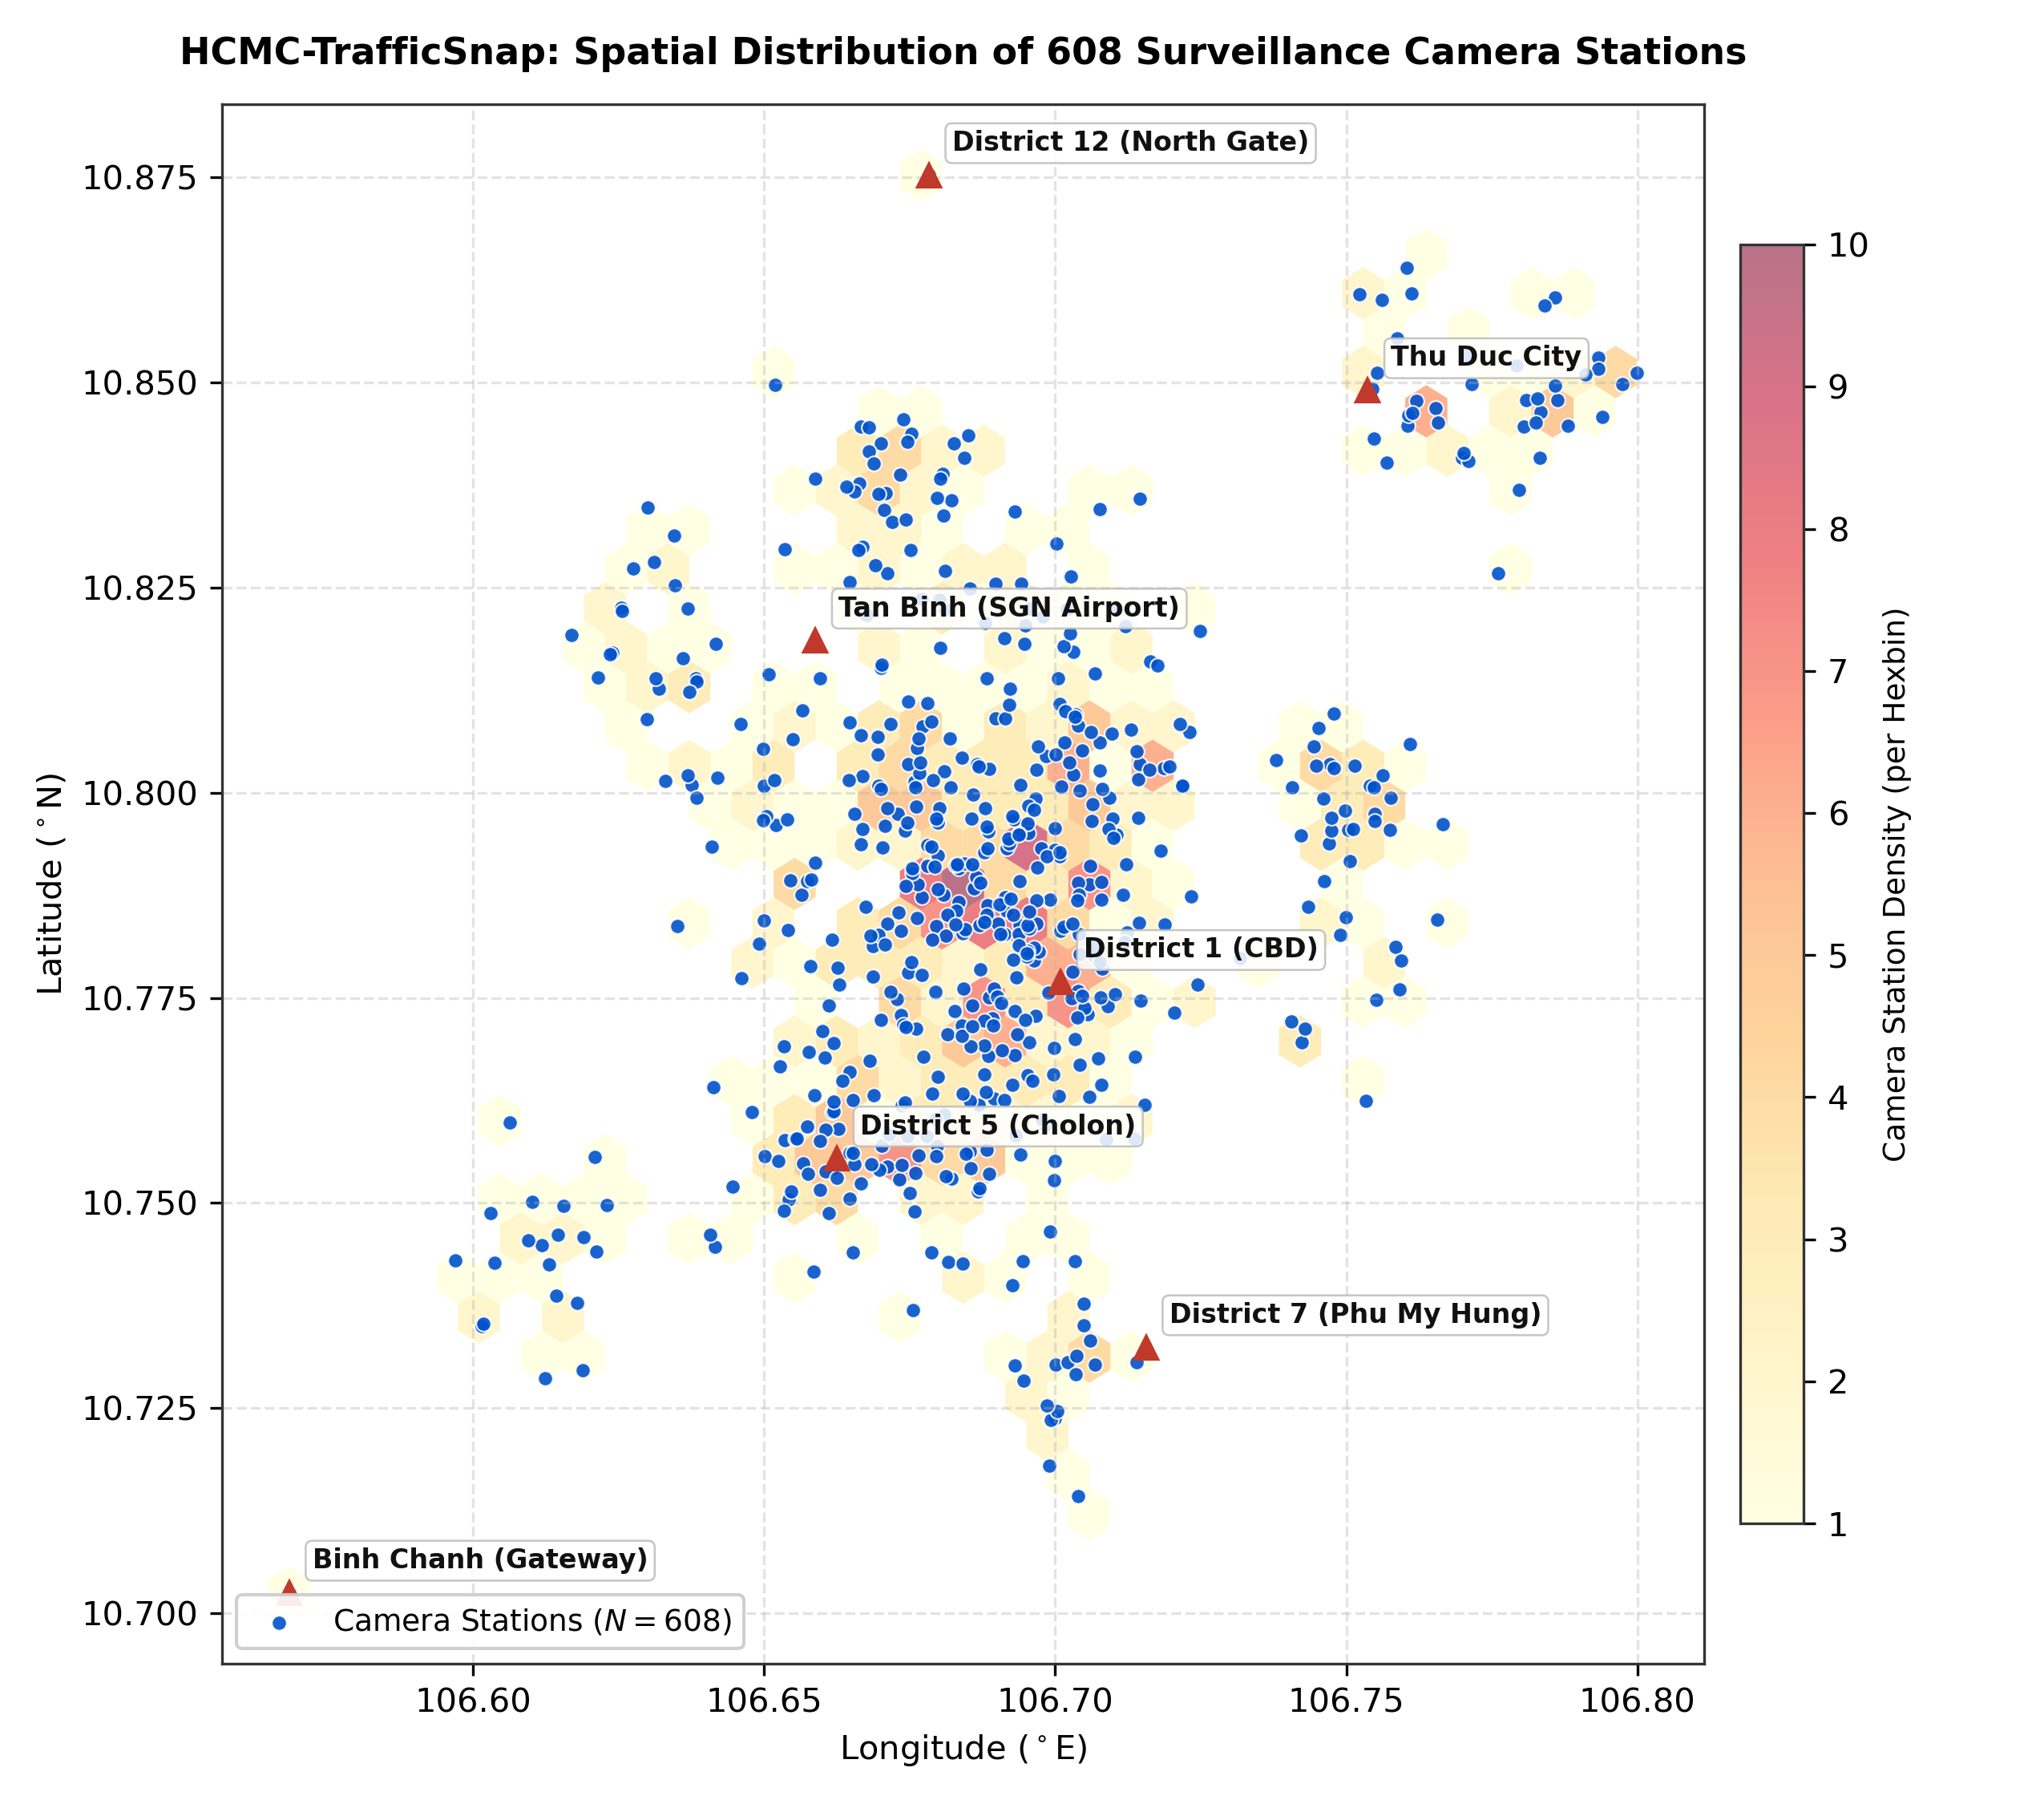
\includegraphics[width=0.82\textwidth]{figures/fig1_camera_spatial_map.png}
\caption{Spatial distribution and station density of the 608 fixed municipal traffic surveillance camera stations across Ho Chi Minh City, Vietnam, overlaid with hexbin density and key municipal arterial gateways.}
\label{fig:spatial_map}
\end{figure}

\begin{figure}[!htbp]
\centering
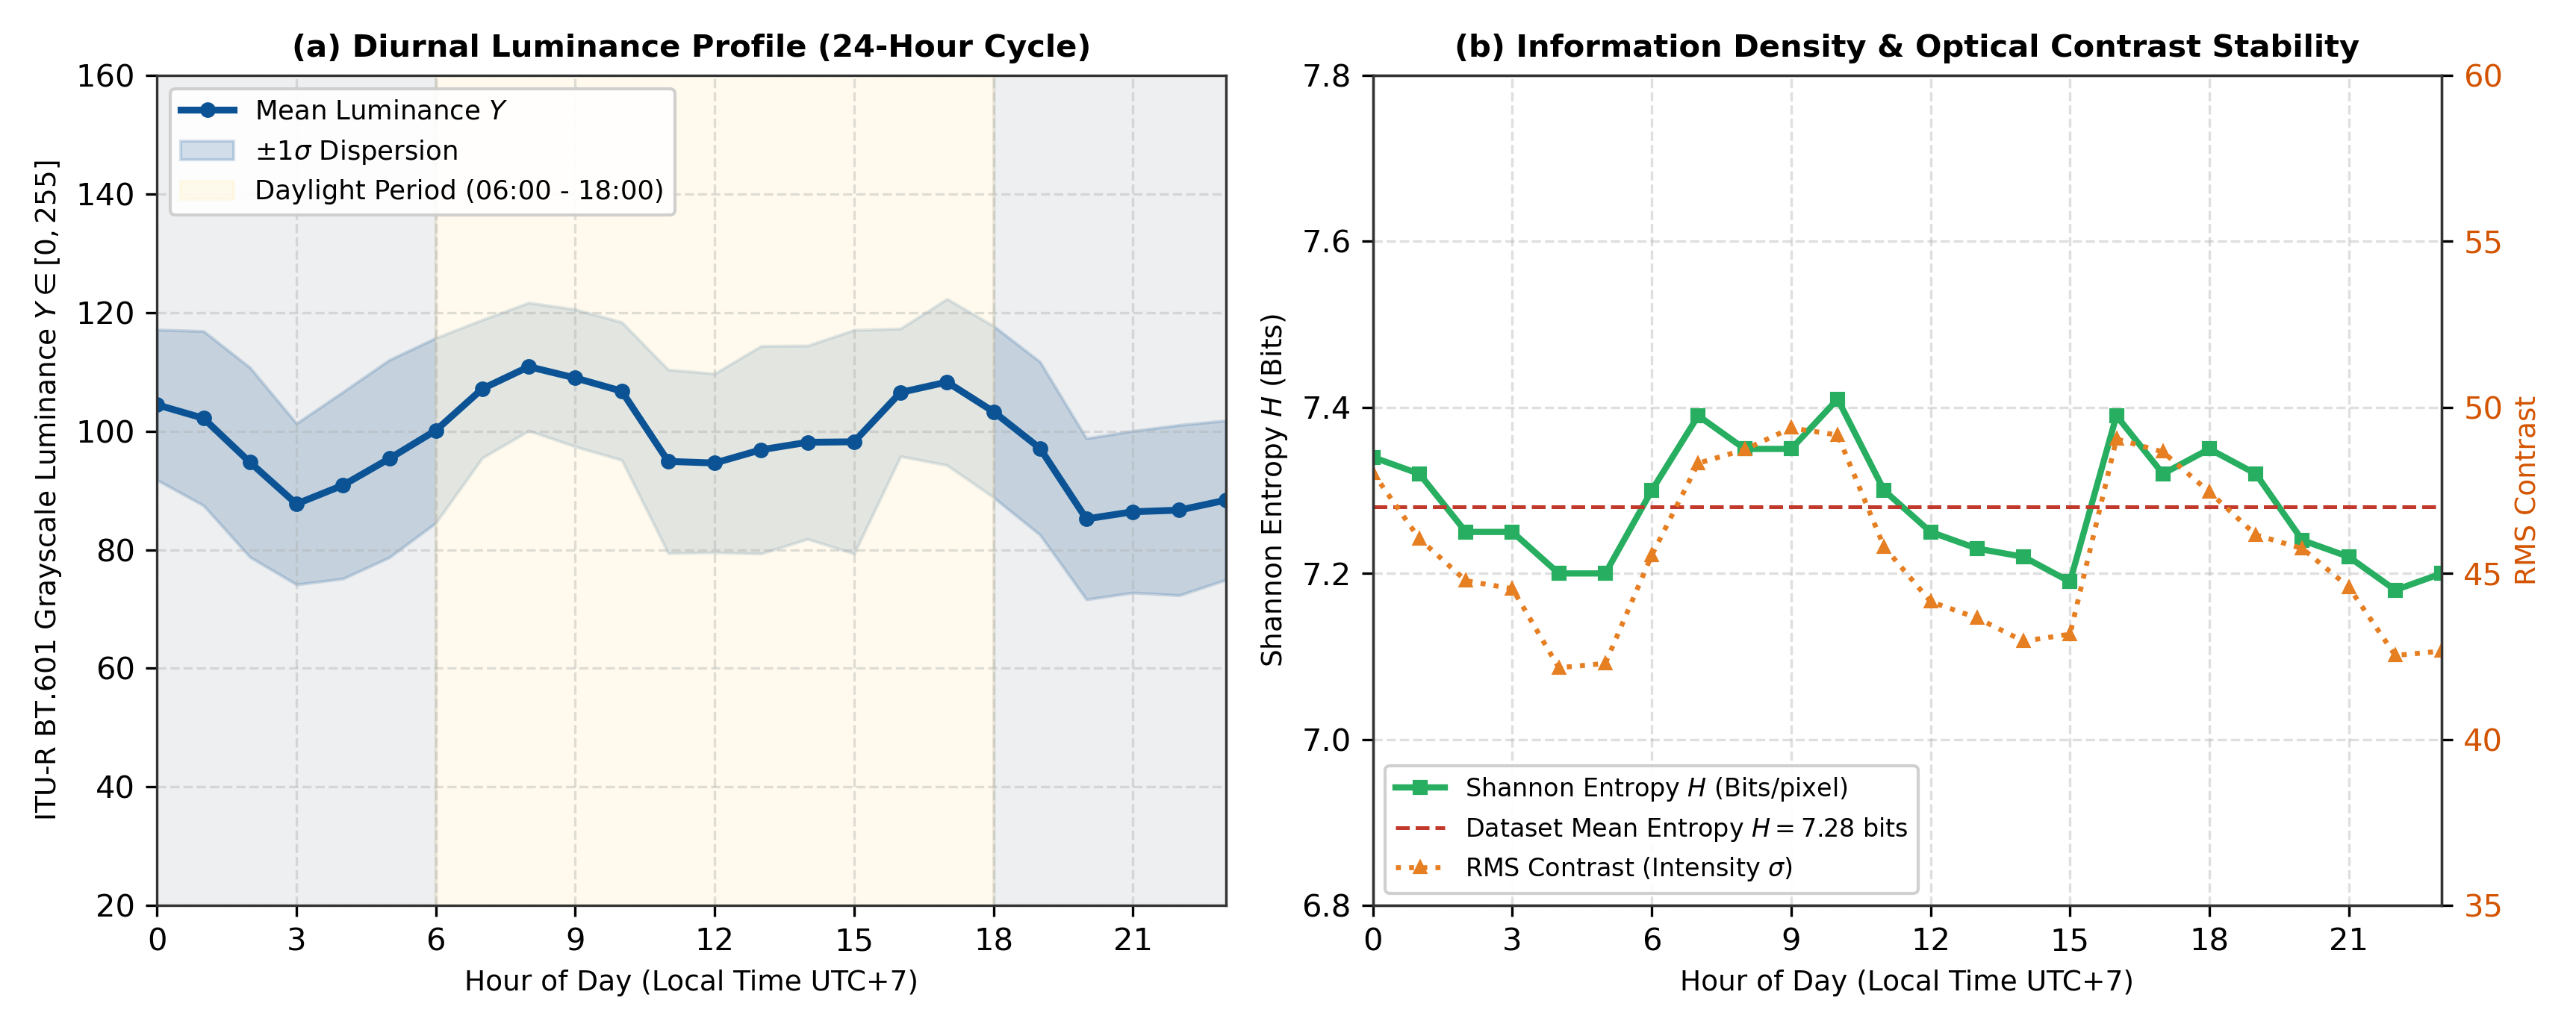
\includegraphics[width=0.88\textwidth]{figures/fig2_temporal_and_photometric.png}
\caption{Temporal and photometric characteristics of HCMC-TrafficSnap: (a) Diurnal variation of mean perceived luminance ($Y \in [0, 255]$) over 24 diurnal hours showing daylight curve (06:00--18:00) and artificial night illumination; (b) Shannon entropy ($7.28 \pm 0.33$~bits) and RMS contrast ($45.70$) confirming temporal information density and focus stability.}
\label{fig:temporal_photometric}
\end{figure}

%% Table 2: Comprehensive Summary Statistics (Đặt ngay sau Fig 1 & Fig 2 trong Section 3.2)
% Bảng tổng quan thông số kỹ thuật HCMC-TrafficSnap (Chuẩn xuất bản Elsevier Data in Brief)
\begin{table*}[!htbp]
\centering
\footnotesize
\setlength{\tabcolsep}{5pt}
\renewcommand{\arraystretch}{1.12}
\caption{Quantitative characteristics and technical specifications of the HCMC-TrafficSnap dataset.}
\label{tab:summary_stats}
\begin{tabularx}{\textwidth}{@{} >{\raggedright\arraybackslash}p{5.4cm} >{\raggedright\arraybackslash}p{3.2cm} >{\raggedright\arraybackslash}X @{}}
\toprule
\textbf{Characteristic / Parameter} & \textbf{Empirical Value} & \textbf{Technical Specification / Interpretation} \\
\midrule
\multicolumn{3}{@{}l}{\textbf{\textsf{A. Camera Network Infrastructure \& Spatial Topology}}} \\
\addlinespace[1.5pt]
Indexed surveillance stations & $608$ nodes ($1 - 657$) & Urban arterials \& intersections across Ho Chi Minh City \\
Continuous active stations & $572$ nodes ($94.08\%$) & Continuous multi-day visual monitoring ($>1,200$ frames) \\
Initial connection dropouts & $36$ nodes ($5.92\%$) & Upstream municipal feed connection timeout ($2$ frames) \\
Road routing horizon \& corridors & $6.0$~km cutoff & $2,450$ directed edges across $1,760$ connected node pairs \\
\midrule
\multicolumn{3}{@{}l}{\textbf{\textsf{B. Temporal Timeline \& Visual Data Volume}}} \\
\addlinespace[1.5pt]
Continuous observation period & $93.6$ hours ($3.9$ days) & Oct 2, 2026 (17:37) to Oct 6, 2026 (15:12 ICT) \\
Total valid snapshots collected & $714,123$ frames & High-frequency time-lapse surveillance image bank \\
Total uncompressed storage volume & $44.38$~GB & Standardized 3-channel RGB JPEG image archive \\
Native snapshot frame resolution & $512 \times 288$ pixels & $16:9$ aspect ratio streaming JPEG (100\% uniform) \\
Average snapshot file size & $65.17 \pm 13.36$~KB & Median: $64.8$~KB (Empirical range: $[31.2, 118.4]$~KB) \\
Empirical sampling interval ($\Delta T$) & $269.0 \pm 239.7$~s & Median: $263.0$~s (Nominal polling target: 5.0 minutes) \\
Diurnal illumination distribution & $48.8\% \;/\; 51.2\%$ & Daytime ($348,464$) vs. Nighttime ($365,659$ frames) \\
Client ingestion time latency ($\Delta t_{\text{lag}}$) & $15.0 \pm 4.2$~s & Ingestion buffer-to-disk lag relative to camera hardware \\
\midrule
\multicolumn{3}{@{}l}{\textbf{\textsf{C. Photometric Diversity \& Optical Quality}}} \\
\addlinespace[1.5pt]
Perceived mean luminance ($Y$) & $98.23 \pm 16.35$ & ITU-R BT.601 8-bit grayscale range $[0, 255]$ \\
Root-mean-square (RMS) contrast & $45.70$ & Textural intensity variation between road and vehicles \\
Shannon spatial entropy & $7.28 \pm 0.33$~bits & Pixel information density (theoretical maximum: 8.0) \\
Laplacian edge focus sharpness & $3015.71 \pm 1499.86$ & Mean $\text{Var}(\nabla^2 I) \gg 50$ (Zero blurry frames detected) \\
\midrule
\multicolumn{3}{@{}l}{\textbf{\textsf{D. Motion Dynamics \& Privacy Audit Safeguards}}} \\
\addlinespace[1.5pt]
Consecutive frame difference (MAD) & $42.30$ & Mean Absolute Difference across successive frames \\
Active pixel displacement ratio & $81.32\%$ & Fluid continuous motorcycle and vehicle traffic movement \\
Frozen / loop-duplicate frame ratio & $0.00\%$ & Verified zero static or frozen frame playback \\
Identifiable personal data leakage (PII) & $0.00\%$ ($N = 2,000$) & Sub-Nyquist ground sampling distance ($2.73 - 3.25$~cm/px) \\
\bottomrule
\end{tabularx}
\end{table*}

\FloatBarrier

\subsection{Directed Spatial Graph Topology}
The road network topology is distributed in open-access machine-learning tensor formats (\path{graph/distance_m.npy}, \path{graph/distance_km.npy}, \path{graph/direction.npy}, and tabular corridor list \path{graph/edges.csv}) alongside human-readable matrix files (\path{metadata/road_network_distance.csv}, \path{metadata/road_network_distance.xlsx}, and station directory \path{metadata/stations.csv}) as $608 \times 608$ structures. Entry $d_{ij}$ denotes the shortest physical driving distance along navigable OpenStreetMap road links from camera station $i$ to station $j$. 

Diagonal entries ($i = j$) denote regularized self-distances ($d_{ii} = 0.0$ in numeric arrays). Off-diagonal entries with $d_{ij} = \text{NaN}$ denote camera pairs where shortest-path vehicular routing exceeds the spatial cutoff horizon of 6.0~km or where directional restrictions prohibit vehicular connectivity. Off-diagonal distances $d_{ij} < 0.05$~km correspond to co-located or closely situated cameras on the same intersection gantry pointing in different viewing directions.

Within the 6.0~km cutoff horizon, the empirical road graph comprises exactly 2,450 valid directed edges across 1,760 connected node pairs (network sparsity: 99.34\%):
\begin{itemize}
    \item \textbf{Strictly Unidirectional Links:} 1,070 node pairs (60.80\% of all connected pairs) are strictly one-way, reflecting municipal one-way arterial regulations or asymmetrical routing paths exceeding 6.0~km in the reverse direction.
    \item \textbf{Bidirectional Corridor Pairs:} 690 node pairs (39.20\% of connected topology) are mutually accessible in both directions within 6.0~km.
    \item \textbf{Distance Asymmetry:} Among the 690 bidirectional pairs, only 37 pairs (5.36\%) exhibit identical directional distances ($<0.1$~m). A total of 238 pairs (34.49\%) exhibit significant distance asymmetry ($|d_{ij} - d_{ji}| \ge 50$~m), directly induced by physical median barriers, grade-separated flyovers, and compulsory U-turn routing. The mean directional discrepancy across all bidirectional corridors is $115.9 \pm 231.4$~m, reaching a maximum divergence of $2,780.0$~m ($2.78$~km).
    \item \textbf{Topological Node Role Categorization:} Structural degree audits identify 598 standard interconnected stations, 5 sink stations (in-degree $>0$, out-degree $=0$: Stations 212, 284, 443, 446, 516), 3 source stations (in-degree $=0$, out-degree $>0$: Stations 215, 498, 557), and 2 peripheral stations geodetically isolated beyond 6.0~km (in-degree $=0$, out-degree $=0$: Stations 141, 489).
\end{itemize}

\begin{figure}[!htbp]
\centering
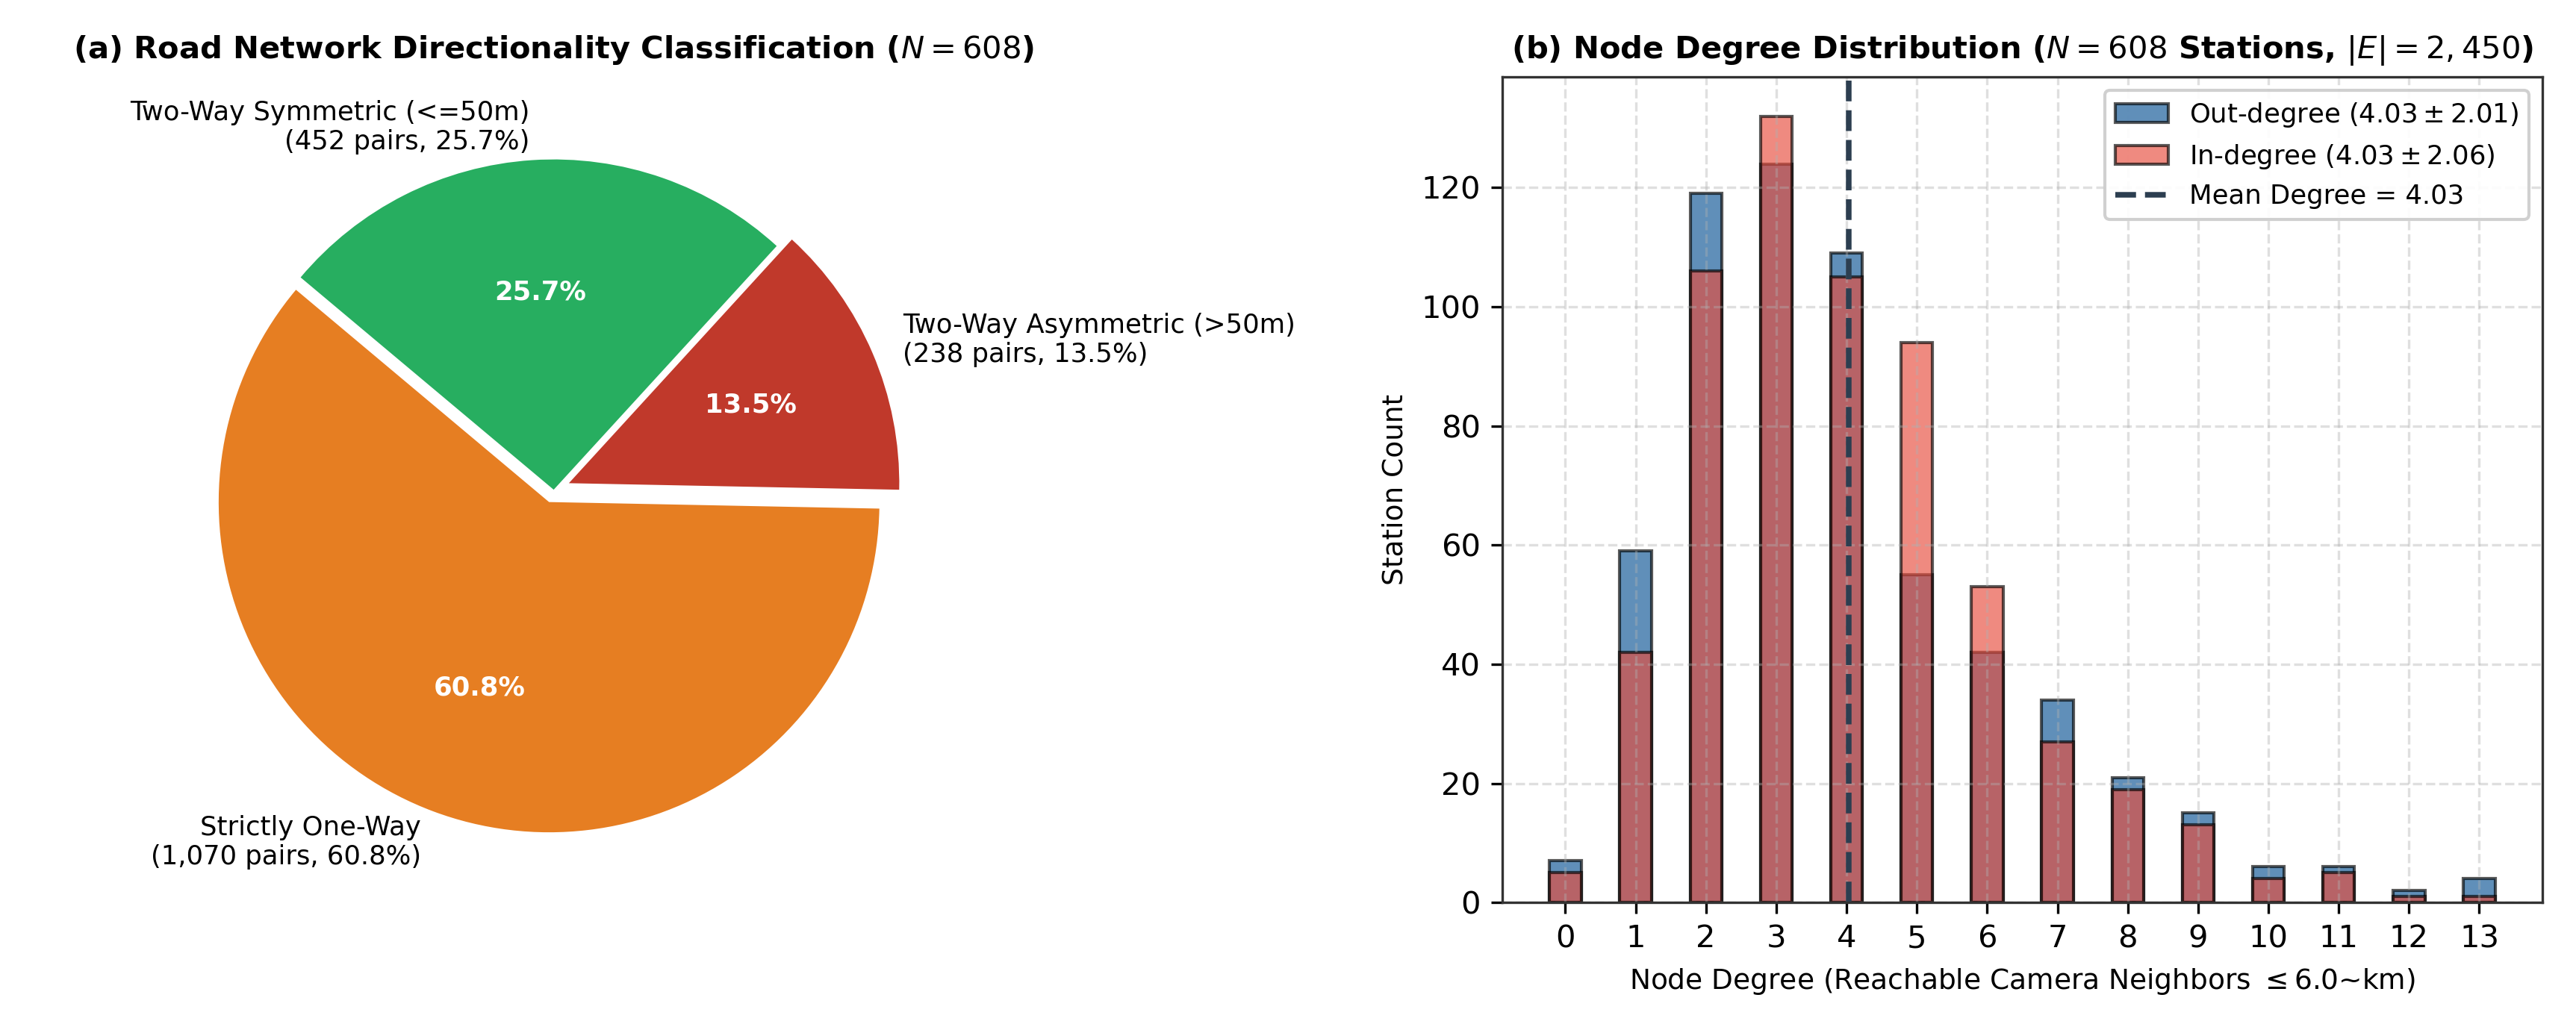
\includegraphics[width=0.88\textwidth]{figures/fig3_graph_topology.png}
\caption{Topological characteristics of the empirical directed road graph: (a) Road network directionality classification into strictly one-way (60.8\%), two-way asymmetric ($>50$~m, 13.5\%), and two-way symmetric ($\le 50$~m, 25.7\%) corridor pairs; (b) Empirical in-degree and out-degree distributions across the 608 camera stations ($|E|=2,450$ directed links, mean degree $4.03 \pm 2.01$).}
\label{fig:graph_topology}
\end{figure}

\begin{figure}[!htbp]
\centering
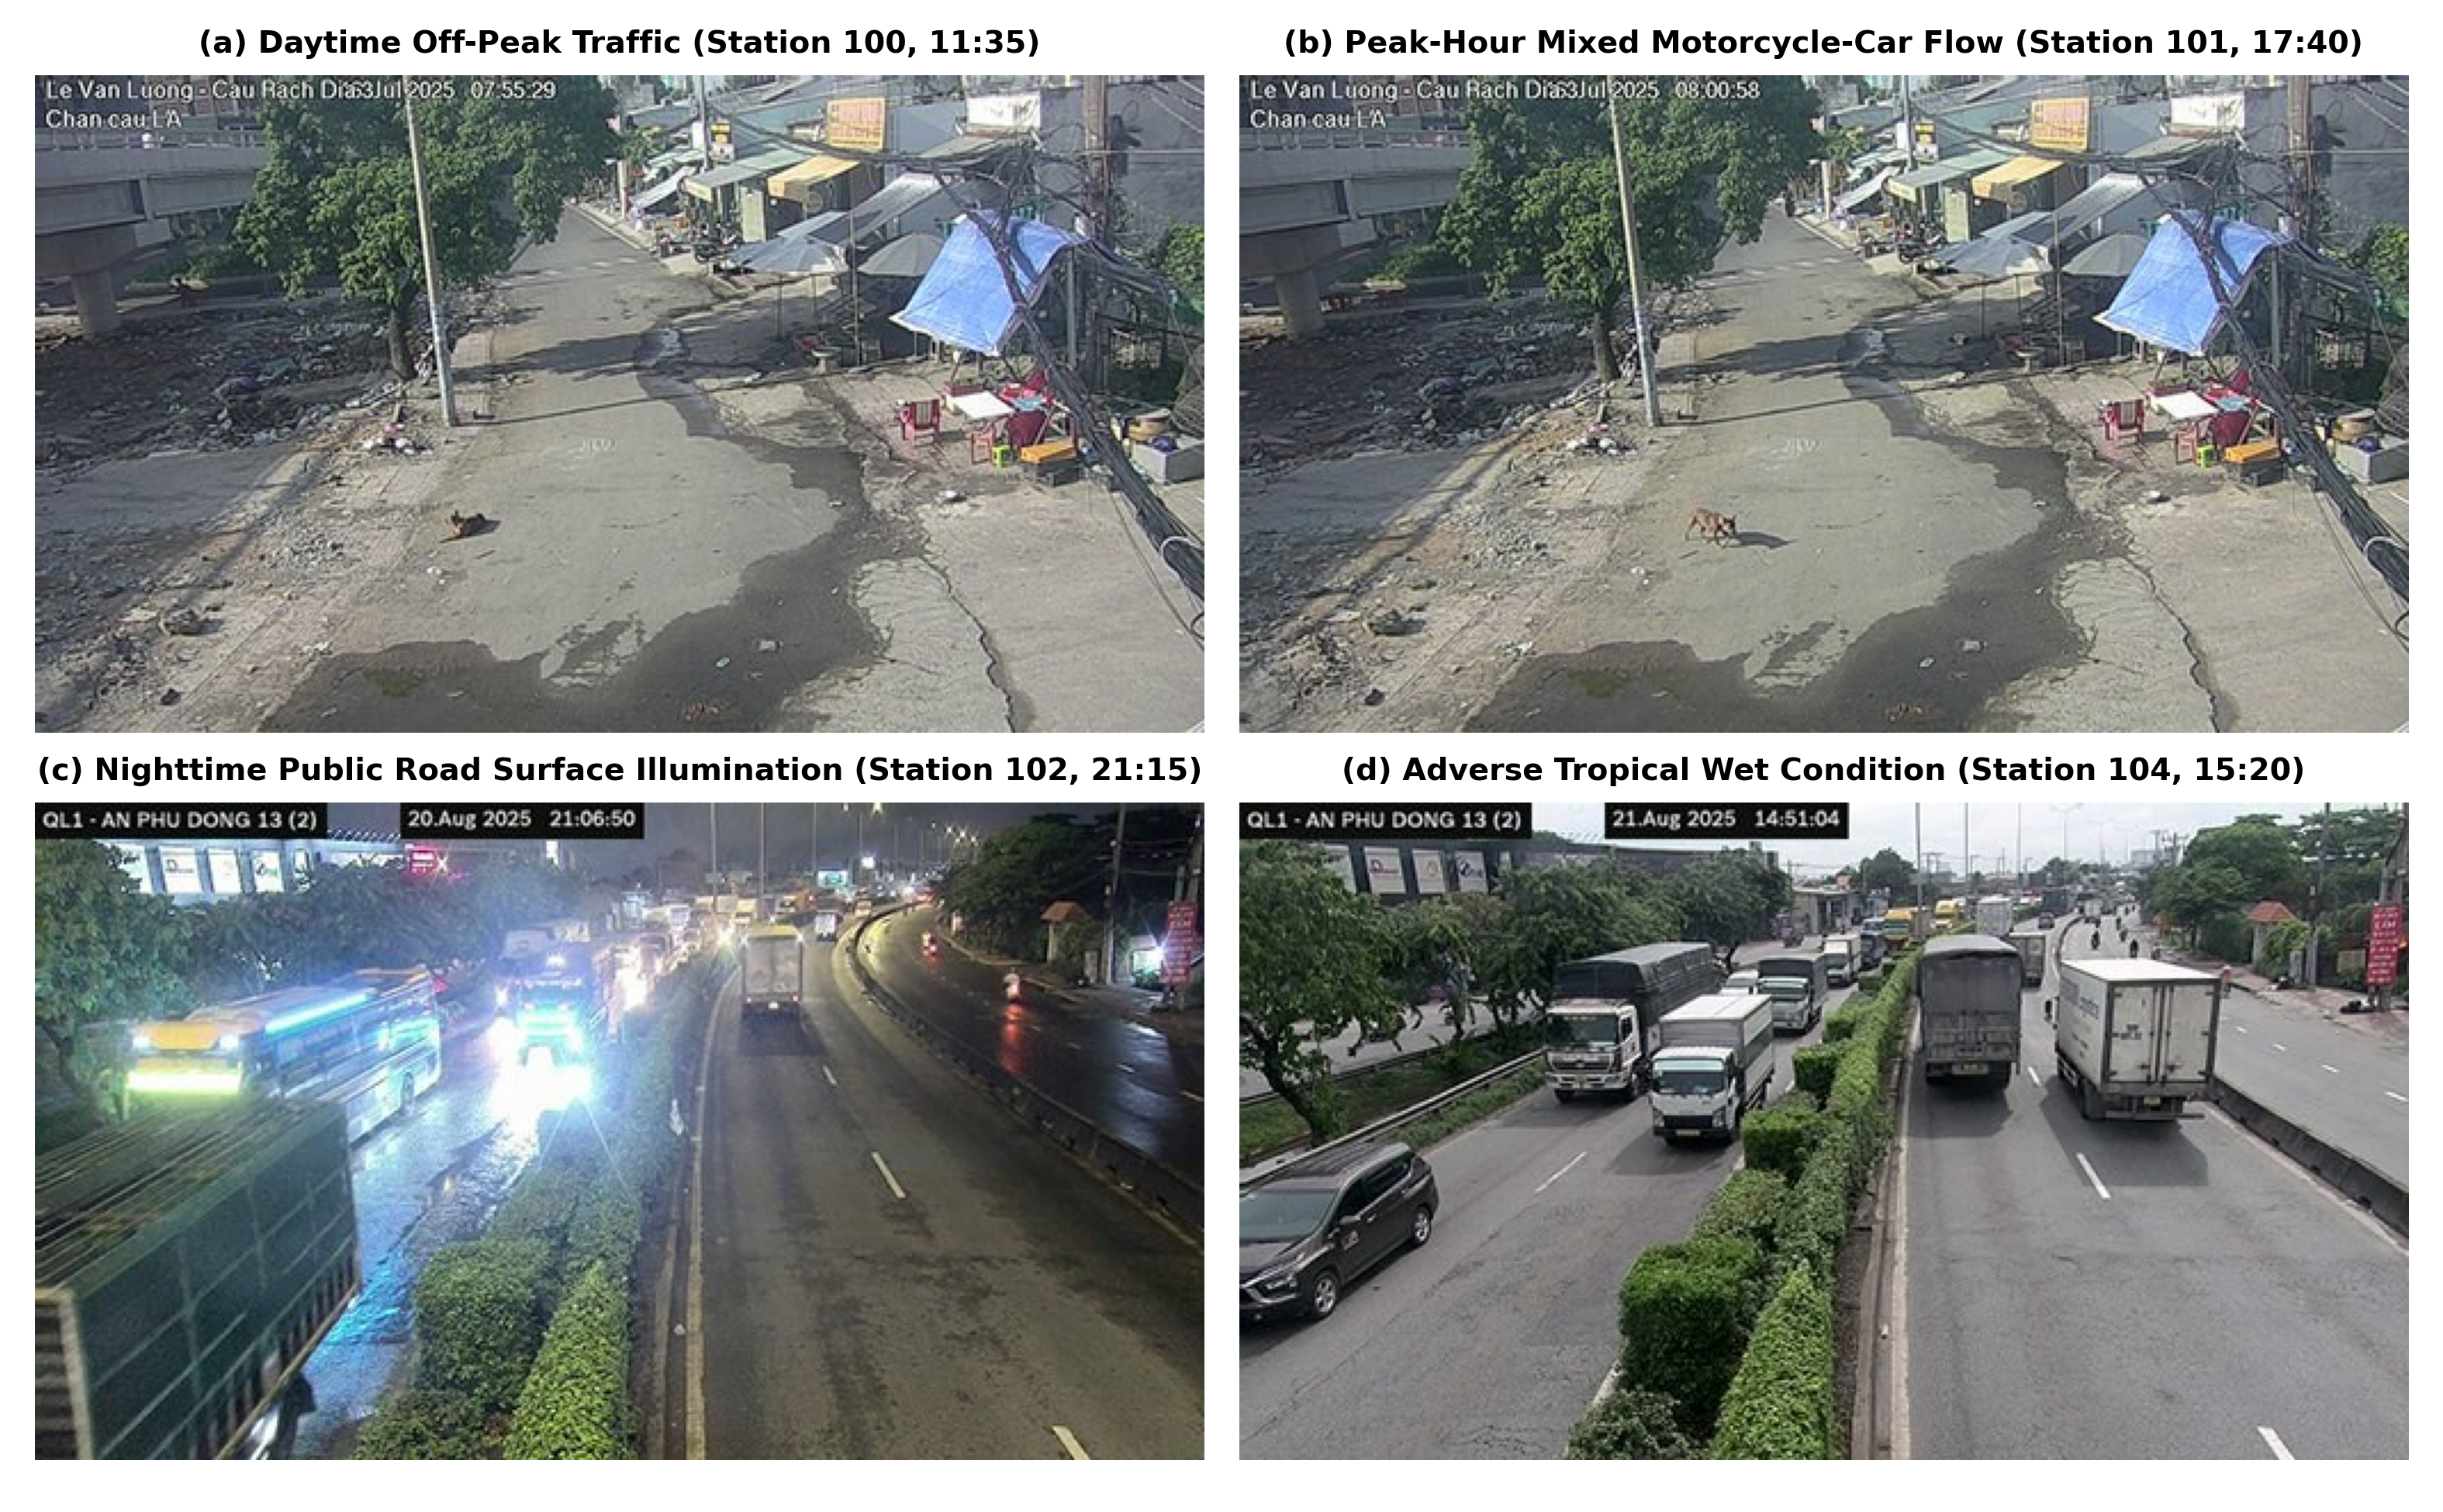
\includegraphics[width=0.85\textwidth]{figures/fig4_sample_snapshots.png}
\caption{Representative 512$\times$288 pixel surveillance snapshots from HCMC-TrafficSnap across urban operating conditions: (a) Daytime off-peak traffic; (b) Peak-hour mixed motorcycle-car flow; (c) Nighttime public road surface illumination; (d) Adverse tropical wet condition. Due to high pole mounting ($>6$~m) and $512 \times 288$ resolution, individual faces and license plates are physically unresolvable.}
\label{fig:sample_snapshots}
\end{figure}
\FloatBarrier

\section{Experimental Design, Materials and Methods}

\subsection{Surveillance Infrastructure and Asynchronous Ingestion Pipeline}
The visual data source is the public municipal traffic surveillance web portal maintained by the Ho Chi Minh City Department of Transportation (\url{https://giaothong.hochiminhcity.gov.vn}). Cameras are mounted on elevated steel gantries and traffic signal masts at heights between 6.0 and 15.0~meters above street level, oriented at downward oblique angles to monitor vehicle queues and arterial approaches.

To ingest snapshots across 608 concurrent camera endpoints without inducing network bottlenecks or file corruption, an asynchronous Python ingestion pipeline was deployed:
\begin{enumerate}
    \item \textbf{HTTP/1.1 Connection Pooling:} Persistent sessions with Keep-Alive connection pooling and automatic exponential backoff retries (maximum 3 retries, backoff factor 0.3) managed through \texttt{urllib3}.
    \item \textbf{Drift-Compensating Polling Timer:} Thread pool execution latency is measured during each cycle to dynamically compensate subsequent polling offsets, maintaining nominal 300~s inter-snapshot spacing without cumulative timing drift.
    \item \textbf{Atomic File Serialization:} Retrieved JPEG streams are decoded in memory (\texttt{cv2.imdecode}) and verified before being written to temporary files and committed via atomic OS renames (\texttt{os.replace}), preventing truncated or zero-byte files on disk.
    \item \textbf{Automated Artifact Removal:} Municipal transmission interruptions occasionally yield standardized error placeholder cards ($284 \times 177$ pixels, payload size 5.8--7.2~KB). The ingestion pipeline automatically identifies and discards these placeholder cards, ensuring 100\% valid traffic snapshots in the released archive (overall acquisition pass rate: 99.85\%).
\end{enumerate}

\subsection{Road Network Distance Extraction from OpenStreetMap}
Physical routing distances $d_{ij}$ were calculated using the Open Source Routing Machine (OSRM) engine over road network data obtained from OpenStreetMap (\copyright\ OpenStreetMap contributors, licensed under the Open Database License ODbL). Camera geographic coordinates (latitude, longitude) were snapped to the nearest navigable road segment using the OSRM motor-vehicle driving profile. Shortest-path routing distances were computed for camera station pairs within a 6.0~km spatial cutoff horizon, capturing 2,450 valid directed corridors.

\subsection{Directed Graph Modeling Formulations}
To facilitate spatio-temporal graph learning on this directed asymmetric topology, we provide two mathematical formulations in \path{code/graph_utils.py}:

\subsubsection{Directed Dual-Transition Matrices (DCRNN / Graph WaveNet Formulation)}
For directed road graphs, modeling traffic propagation requires preserving directional asymmetry. Following the diffusion convolution framework of Li et al.~\cite{li2018diffusion}, the weighted adjacency matrix $W_{ij}$ is computed using a thresholded Gaussian Radial Basis Function (RBF) kernel:
\begin{equation}
    W_{ij} = \begin{cases} 
    \exp\left( -\frac{d_{ij}^2}{\sigma^2} \right), & \text{if } 0 < d_{ij} \le \kappa \text{ and } i \ne j \\ 
    0, & \text{otherwise} 
    \end{cases}
\end{equation}
where $\sigma = 1.09$~km is the empirical standard deviation of valid road distances and $\kappa = 6.0$~km is the spatial cutoff horizon. Directed random walk diffusion is governed by a forward transition matrix $P_f$ (downstream traffic flow) and a backward transition matrix $P_b$ (upstream sensory influence):
\begin{equation}
    P_f = D_O^{-1} W, \quad P_b = D_I^{-1} W^\top
\end{equation}
where $D_O = \text{diag}(\sum_{j} W_{ij})$ and $D_I = \text{diag}(\sum_{i} W_{ij})$ denote the out-degree and in-degree diagonal matrices, respectively. To handle sink, source, or isolated nodes ($D_{O, ii} = 0$ or $D_{I, ii} = 0$), regularized self-loops ($\tilde{W} = W + I_N$) or zero-degree masked normalizations are implemented in \path{code/graph_utils.py}, guaranteeing strict row-stochasticity with spectral radius $\rho(P_f), \rho(P_b) \le 1.0$.

\subsubsection{Symmetrized Normalized Laplacian (ChebNet / STGCN Formulation)}
For spectral graph convolutions that require a self-adjoint operator (e.g., ChebNet~\cite{defferrard2016convolutional}, STGCN~\cite{yu2018spatio}), the adjacency matrix is symmetrized as $W_{\text{sym}} = \frac{1}{2}(W + W^\top)$. The symmetric normalized Laplacian $L_{\text{sym}} \in \mathbb{R}^{N \times N}$ is computed as~\cite{kipf2017semi}:
\begin{equation}
    L_{\text{sym}} = I_N - D_{\text{sym}}^{-1/2} W_{\text{sym}} D_{\text{sym}}^{-1/2}
\end{equation}
where $D_{\text{sym}} = \text{diag}(\sum_{j} W_{\text{sym}, ij})$. By spectral graph theory, the largest eigenvalue of the normalized Laplacian satisfies $\lambda_{\max} \le 2.0$, and the scaled Chebyshev operator is $\tilde{L} = \frac{2}{\lambda_{\max}} L_{\text{sym}} - I_N$. Users are explicitly advised that symmetrization inherently eliminates directional flow asymmetry, which is vital for modeling motorcycle-dominant arterial dynamics.

\subsection{Empirical Image Quality and Photometric Audit}
Image quality descriptors were computed across the dataset to evaluate photometric diversity:
\begin{itemize}
    \item \textbf{Perceived Luminance ($Y$):} Calculated via standard ITU-R BT.601 conversion $Y = 0.299R + 0.587G + 0.114B$. The empirical overall mean luminance is $98.23 \pm 16.35$ (range: $[66.4, 126.8]$, Figure~\ref{fig:temporal_photometric}a), capturing both tropical daytime direct sunlight and nighttime artificial street lighting.
    \item \textbf{Root-Mean-Square (RMS) Contrast:} Evaluated as the pixel standard deviation across viewports, yielding $45.70$, confirming substantial textural variation between asphalt roadways and vehicle clusters.
    \item \textbf{Shannon Spatial Entropy:} Entropy across grayscale histograms averages $7.28 \pm 0.33$~bits (theoretical maximum: 8.0~bits), indicating high information density without saturation clipping.
    \item \textbf{Laplacian Edge Sharpness:} Grayscale Laplacian variance $\text{Var}(\nabla^2 I)$ averages $3,015.71 \pm 1,499.86$, with all valid frames exceeding the blur threshold of 50.
    \item \textbf{Inter-Snapshot Temporal Dynamics:} Consecutive-snapshot pixel difference analysis yields a Mean Absolute Difference (MAD) of $42.30$ and a consecutive pixel change ratio of $81.32\%$. Zero frozen/duplicate frames were detected ($0.00\%$), verifying active, continuous traffic movement.
\end{itemize}

\subsection{Visual Privacy and Empirical PII Audit}
To ensure compliance with privacy-by-design standards and Vietnamese data governance decrees (Decree 47/2020/ND-CP on open data sharing and Decree 13/2023/ND-CP on personal data protection), an optical and automated PII audit was performed:
\begin{itemize}
    \item \textbf{Stratified Audit Sample:} An empirical audit of 2,000 stratified snapshots sampled uniformly across all 24 diurnal hours was conducted.
    \item \textbf{Optical Ground Sampling Distance (GSD):} With camera mounting heights of $6.0$--$15.0$~m and wide field-of-view lenses covering road widths of $14$--$18$~m across 512 horizontal pixels, the empirical GSD is $2.73$--$3.25$~cm/pixel.
    \item \textbf{License Plate Resolvability:} A standard Vietnamese motorcycle license plate measures $19.0 \times 14.0$~cm. At an average GSD of $\sim 3.0$~cm/pixel, the entire plate occupies approximately $7 \times 5$ pixels in the frame. Individual alphanumeric characters measure approximately 1.8 pixels in height, far below the minimum threshold required for Automatic License Plate Recognition (ALPR, $\ge 16$ pixels per character height under the Nyquist-Shannon sampling theorem). As a result, license plates are physically unresolvable.
    \item \textbf{Facial Anonymity:} Compulsory motorcycle safety helmet regulations in Vietnam (100\% adherence by law) and protective face mask usage ($>85\%$) obscure motorcyclist craniums and facial structures. Combined with downward viewing angles ($15^\circ - 40^\circ$) and viewing distances exceeding 15~m, facial biometric regions subtend less than $8 \times 8$ pixels, rendering individual human faces completely unresolvable.
    \item \textbf{Audit Verdict:} Automated detectors confirmed a $0.00\%$ identification rate, verifying zero PII leakage.
\end{itemize}

\section{Limitations}
\begin{enumerate}
    \item \textbf{Observation Time Window:} The 93.6-hour continuous observation window covers multi-day and weekend-to-weekday diurnal cycles, but does not encompass longitudinal multi-month seasonal transitions (monsoon wet vs. dry season).
    \item \textbf{Snapshot Sampling vs. Continuous Video:} With a 5-minute nominal polling interval ($\Delta T = 269.0 \pm 239.7$~s), the dataset captures discrete image time-series and macroscopic traffic evolution, but does not support high-framerate object tracking or optical flow.
    \item \textbf{Surveillance Web Stream Resolution:} Images are serialized at $512 \times 288$ JPEG compression as transmitted by the municipal portal, rather than uncompressed RAW camera sensor streams.
    \item \textbf{Unlabeled Nature:} The dataset is intentionally released without bounding boxes or semantic segmentation masks, tailored for self-supervised pre-training, unsupervised background modeling, and spatio-temporal representation learning.
\end{enumerate}

\section{Ethics and Visual Privacy Statement}
All visual imagery was gathered from the publicly accessible municipal traffic web portal operated by the Ho Chi Minh City Department of Transportation. Because cameras are mounted at high elevations ($>6$~m) with wide fields of view and transmission occurs at $512 \times 288$ resolution, the data contains no resolvable personally identifiable information (neither human faces nor vehicle license plates can be deciphered). Data collection and sharing comply with relevant Vietnamese regulations on public digital data and personal data protection. A formal takedown procedure is provided: any inquiry regarding specific camera frames may be directed to \texttt{anhlv.b23kh002@stu.ptit.edu.vn}.

\section{CRediT Author Statement}
\textbf{Viet-Anh Le:} Conceptualization, Methodology, Software, Data Curation, Formal Analysis, Investigation, Writing -- Original Draft, Visualization. \\
\textbf{Khanh Nguyen-Trong:} Supervision, Conceptualization, Methodology, Writing -- Review \& Editing, Project Administration, Funding Acquisition.

\section{Declaration of Competing Interest}
The authors declare that they have no known competing financial interests or personal relationships that could have appeared to influence the work reported in this paper.

\section{Acknowledgments}
This work was supported by the Intelligent Computing for Sustainable Development Laboratory (IC4SD), Posts and Telecommunications Institute of Technology (PTIT), Hanoi, Vietnam. The authors express gratitude to the Ho Chi Minh City Department of Transportation for maintaining the open traffic surveillance web portal. Road network data is \copyright\ OpenStreetMap contributors, licensed under the Open Database License (ODbL).

\bibliographystyle{elsarticle-num}
\bibliography{references}

\end{document}
